\section{Lung model assumptions}
%\label{sec:model}
%
%
%\subsection{Model assumptions}
\label{sec:assumptions}
%
%We will begin by giving a review of the main modelling assumptions and how they might affect the model's ability to predict deformation and ventilation within healthy and diseased lungs.
%

\subsection{Approximating lung parenchyma using a poroelastic medium}

\noindent \newline \textbf{Averaging over the tissue:} One of the major assumptions is that we can approximate the lung parenchyma using a poroelastic continuum description. This makes our model computationally tractable and allows us to use the well established theory of poroelasticity to couple the air with the tissue.

The use of a continuum model can be further supported by looking at the different length scales and structures of the tissue. For the microscopic length scale denoted by $l$ of the parenchyma we will use the diameter of an alveolus that can be approximated to be $0.02 \; \mbox{cm}$ \cite{ochs2004number}. The macroscopic length scale $L$ can be taken to be the diameter of a segment which measures around $4\;\mbox{cm}$ of tissue. So the ratio of the different length scales is small i.e $\epsilon := \frac{l}{L} \approx 0.005 \ll 1$. This along with the assumption that the structure of an acinus is porous (see Figures \ref{fig:pores} and \ref{fig:honey}) and approximately periodic supports the use of averaging techniques over the tissue to obtain a continuum description  in the form of a poroelastic medium. To further simplify the poroelastic equations we assume that the poroelastic continuum can be described by a solid phase (blood and tissue) and a fluid phase (air), where both phases are assumed to be incompressible. The interaction between the fluid pressure and the deformation of the solid skeleton is assumed to obey the effective stress principle. Note that by averaging over the tissue we do not seek to model individual alveoli but introduce macroscopic parameters such as the permeability and elasticity coefficients. In general, lung diseases usually affect significant regions of alveoli (lung tissue), thus, by changing the macro-scale parameters over the affected area of tissue we are still able to model changes in the tissue due to disease.

\noindent \textbf{Ignoring blood flow:}\label{section:blood_flow} Apart from collagen, fibers and air the other major component in the lung is blood. The volume taken up by collagen and  elastin fibers is similar to the volume occupied by the capillaries filled with blood (illustrated in Figure \ref{fig:pores}). In fact, the space not occupied by air is about $7\%$ of the parenchymal volume and is made up of $50\%$ capillary blood and $50\%$ of collagen and elastin fibers \cite{WeichertThesis}. Also the density of blood is similar to the density of tissue and much larger than that of air ($ {1060 \;\mbox{kg}\,\mbox{m}}^{-3}\gg  {1.18 \;\mbox{kg}\,\mbox{m}}^{-3}$). Since the capillaries are constantly filled with blood and the density of blood is similar to that of alveolar tissue we will make the simplifying assumption that the blood is simply part of the tissue (solid phase) and thus ignore accelerations and any redistribution of blood during breathing.

\noindent \textbf{Assuming incompressibility of the solid and the fluid:} Blood and tissue can be assumed to be incompressible. Under physiological conditions, air can also be assumed to be incompressible \cite{ismail2013coupled}.

\noindent \textbf{Ignoring solid inertia forces:}
\label{section:inertia} Simple calculations considering the sinusoidal motion of tissue near the diaphragm during normal breathing yield an estimate of $0.02\, \mbox{ms} ^{-2}$ for the maximum acceleration of lung parenchyma. Compared to the acceleration of gravity this is negligible, and it is therefore reasonable to ignore the inertia forces in the tissue.

\noindent \textbf{Ignoring fluid inertia forces:}
The fluid's Reynolds number in the lower airways that form part of the lung parenchyma, has been estimated to be around $1$ to $0.01$ \cite{pedley1970prediction}. Due to this relatively low Reynolds number we choose to ignore fluid inertia forces in the poroelastic medium. %\cite{ben2006simplified} also showed in their whole lung model that inertia forces can be neglected during quiet breathing.

\noindent \textbf{Ignoring viscous forces in the fluid:}\label{section:viscous_forces}
A dimensional analysis shows that the viscous stress in the fluid is small compared to the drag forces between the fluid and the porous structure, when the ratio of the different length scales is small \cite{markert2007constitutive}. We will therefore neglect the fluid viscous stress implying that the fluid behaves more or less inviscid within the porous structure.

%The magnitude of the viscous stress in the fluid $\left|\left|\nabla \bb{\sigma}_{visc}\right|\right|$ within a poroelastic medium can be evaluated according to \cite{coussy2004poromechanics} as $\left|\left|\nabla \bb{\sigma}_{visc}\right|\right|= \frac{\phi \mu^{f}}{l L} \left|\left|\bb{v}^{f} - \bb{v}^{s} \right|\right|$,
%where $l$ and $L$ are the microscopic and macroscopic characteristic length scales, respectively. This can be balanced with the order of magnitude of  $\left|\left| \frac{\phi^{2}}{\boldsymbol{k}}  \left(\bb{v}^{f} - \bb{v}^{s}\right)  \right|\right|$ that describes the viscous resistance opposed by the shear stress to the fluid flow from the drag at the internal walls of the porous network. To see whether the viscous forces play an important role we take the ratio between these two forces% as is done in section 3.3.1 of \cite{coussy2004poromechanics}
%\begin{equation*}
%  \left|\left|\nabla \bb{\sigma}_{visc}\right|\right| / \left|\left| \frac{\phi^{2}}{\boldsymbol{k}}  \left(\bb{v}^{f} - \bb{v}^{s}\right)  \right|\right|=\frac{\mu_{f} \boldsymbol{k} }{ \phi l L}.
%  \label{viscous_balance}
%\end{equation*}
%Using parameter estimates for healthy human tissue found in Table \ref{tab:lung_sim_parameters}, and the previous estimates of the length scales, we get a non-dimensional value for (\ref{viscous_balance}) of about $0.002 \ll 1$, indicating that viscous forces are insignificant. However, if we were to consider diseased states such as emphysema, where large areas of lung tissue completely break down leaving big holes, it could be argued that the permeability here increases by large amounts that would also cause the above estimate to increase, and suggest that in this case viscous forces could well play an important role, making it important to include them in our model. For simplicity we will choose to ignore this viscous stress for now but it may be included it in a future version of the model by replacing the Darcy flow model with a Brinkman, or even a Stokes flow model for big holes, where the homogenization assumption of a porous structure is not valid.
%\newline

%\noindent \textbf{Constitutive laws:}
%For simplicity we use an isotropic hyperelastic strain energy law to model the tissue.
%%
%%An isotropic strain energy law has already successfully been applied to model the tissue deformation in the healthy lung \cite{tawhai2009supine}.
%%
%Note that for diseased cases such as emphysema or fibrosis this isotropic assumption may become invalid. We also assume that the permeability of the tissue is isotropic. Again the assumption of an isotropic permeability may well become invalid during disease. With the increasing availability of detailed imaging data on the structure of the lung along with further modelling work on constitutive laws for lung tissue, anisotropic laws should be used in the future.
%
\begin{comment}
\begin{figure}[h]
  \centering
\subfloat[]{\label{fig:pores}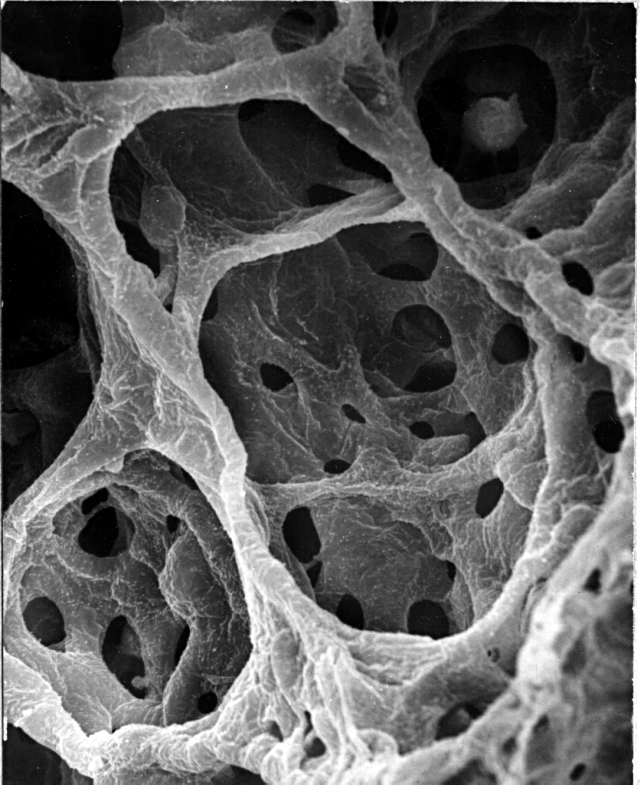
\includegraphics[width=0.35\textwidth,height=2in]{figures/aveolarPores_BerkeleyLungLabLungtour.png}}  \subfloat[]{\label{fig:honey}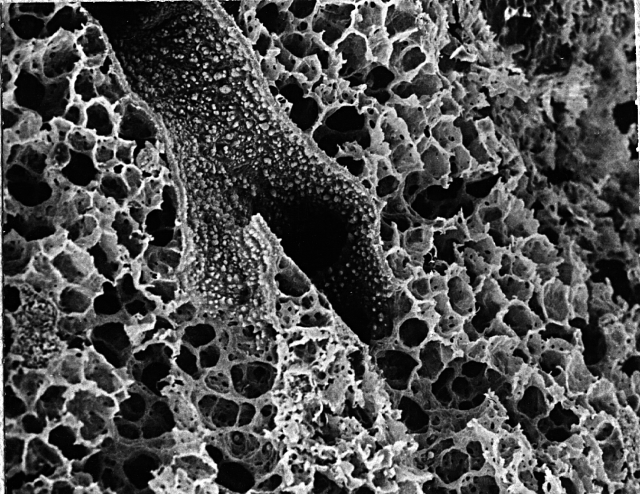
\includegraphics[width=0.35\textwidth,height=2in]{figures/TB_to_aveolarduct_BerkeleyLungLabtour.png}}
\caption{(a) Alveoli in an alveolar duct. The dark round openings are pores between alveoli. The alveolar wall is quite thin and contains a network of capillaries. The average diameter of one alveoli is $0.2\;\mbox{mm}$. (b) Transition from terminal bronchiole to alveolar duct, from conducting airway to oxygen transfer area, diameter of terminal bronchiole is $0.5 \;\mbox{mm}$. Images are reproduced from \cite{lunglabshort}.
 }
   \label{fig:acinar_units}
\end{figure}
%
\end{comment}

\subsection{Approximating the airways using a fluid network model}
%
In order to make the coupled model computationally feasible we assume that a simple laminar flow model can describe the air flow in the airways and we make the common {Poiseuille flow assumption}. This flow assumption is also made in \cite{Swan2012,leary2014effects} where the air flow in a whole airway tree, from trachea down to the final bronchioles was assumed to be governed by Poiseuille flow.  Diseases affecting the airway tree can be modelled effectively by changing resistance (airway radius) parameters in the network flow model.
